%% -*- eval: (flyspell-mode 1); -*-

\chapter{Extraction et formalisation du parallélisme}

Le parallélisme dans un programme informatique est difficile à trouver automatiquement et la plupart du temps il est exprimé explicitement par le développeur. Il est alors nécessaire de lui offrir des outils permettant d'écrire le code parallèle simplement, en lui proposant notamment des fonctions et des mots-clés dans le langage choisi qui sont en accord à la fois avec les besoins matériels et à la fois avec les besoins algorithmiques. Ce chapitre dresse d'abord un état de l'art des principales solutions existantes, puis introduit les principaux objectifs du DSEL développé pendant le stage.

\section{Contexte}

Les applications parallèles sont utilisées depuis un certain nombres d'années afin d'obtenir des performances (en matière de rapidité, et en matière de taille du problème traité). Or il est difficile d'écrire des codes parallèles, ce qui a été évoqué au chapitre précédent. À ce titre divers outils pour faciliter la parallélisation sont apparus, tels que \textsf{ParaScope} dès $1989$ \cite{Art24} qui est éditeur de code interactif. Ces outils se décomposent en de nombreuses catégories à la fois par rapport aux utilisateurs qu'ils visent, et à la fois par rapport au parallélisme qu'ils permettent. En seconde partie sont introduits Les stencils, qui constituent la classe de problèmes étudiée pendant ce stage, et permettent de rappeler la hiérarchie du matériel. 

\subsection{Expression du parallélisme}

Décrire les problèmes à résoudre et le parallélisme qu'ils peuvent utiliser peut se faire de différentes manières avec les moyens actuels. Notamment il est possible de regrouper quatre catégories qui sont les langages dédiés aux scientifiques (non spécialistes du HPC), les langages et compilateurs pour les développeurs de métier (mais non obligatoirement spécialistes du HPC), l'ensemble des bibliothèques et supports d'exécution spécialisés (destinés aux spécialistes du HPC), et en enfin les outils de formalisation des algorithmes employés (destinés aux spécialistes du HPC).

\paragraph{Langages dédiés aux scientifiques.}
Les langages dédiés aux scientifiques sont la plupart du temps des outils de simulation à destination d'experts dans ce domaine. Dans le cas des mathématiques par exemple, de nombreux logiciels définissant leur propre langage existent : \textsf{\href{http://www.wolfram.com/mathematica/}{Mathematica}}, \textsf{\href{http://fr.mathworks.com/}{MATLAB}} ou encore \textsf{\href{http://pari.math.u-bordeaux.fr/}{PARI/GP}} ; et une partie de leurs algorithmes sont parallélisés (au moins au niveau d'un processeur) pour des raisons de performances. Des initiatives plus poussées du côté du parallélisme sont également présentes en recherche comme \textsf{QIRAL} \cite{Art13,Art14} qui à partir d'algorithmes décrits en \LaTeX permet de générer un code parallèle optimisé pour les processeurs des ordinateurs courants -- mais pas pour les supercalculateurs --, il se base pour cela sur le système de réécriture \textsf{Maude} \cite{Art12}. La logique est alors la suivante : offrir à l'utilisateur les mêmes fonctions qui sont connues dans son domaine, en cachant l'implantation et la parallélisation de ces fonctions (telles qu'un calcul de facteurs premiers par exemple).

\paragraph{Langages dédiés au parallélisme.}
Quant il s'agit de développeurs souhaitant écrire du code parallèle sans forcément connaître les subtilités des machines d'exécutions, différents langages spécifiques ont été créés. De manière générale il s'agit en fait d'un langage déjà connu (\textsf{Java} ou \textsf{C/C++}) auquel sont ajoutés quelques mots-clés ou éléments de syntaxes (souvent pour les tableaux notamment) ; \textsf{\href{http://chapel.cray.com/}{Chapel}}, \textsf{\href{https://www.cilkplus.org/}{Cilk}}, \textsf{\href{http://upc.lbl.gov/}{UPC}}, \textsf{Lime} \cite{Art8}, \textsf{\href{http://x10-lang.org/}{X10}} et le langage proposé dans\cite{Art10} rentrent dans cette catégorie. Alors que les trois premiers cités sont très proches des langages d'origines, les trois derniers sont plus éloignés et proposent des paradigmes différents (comme les Map/Reduce dans \textsf{Lime} ou les horloges dans \textsf{X10}). Avec ces langages viennent souvent les compilateurs associés, toutefois parfois il s'agit plus simplement de réécriture automatique de code (vers un langage déjà existant) comme proposé par \textsf{Par4All} \cite{Ths2}. \textsf{Par4All} peut d'ailleurs être considéré comme un éditeur de code dédié au parallélisme, de même que le projet \textsf{Eclipse \href{http://www.eclipse.org/ptp/}{PTP}} (Parallel Tools Platform) ou les projets présentés dans les articles \cite{Art23,Art25}. Ces éditeurs rassemblent alors généralement plusieurs outils, et sont plus interactifs, mais leur parallélisation n'est pas toujours optimale.

\paragraph{Bibliothèques spécialisées.}
Pour atteindre un parallélisme optimal il est souvent nécessaire de descendre à un niveau plus proche du matériel. Plutôt que d'introduire quelques mots-clés supplémentaires, il s'agit alors de plusieurs dizaines de fonctions regroupées dans des bibliothèques. Il faut alors parfois utiliser différentes bibliothèques afin de gérer les différents niveaux de parallélisme (notamment interprocesseur et intraprocesseur). La bibliothèque utilisée dans le cadre du stage en fait partie : \textsf{\href{https://www.khronos.org/sycl}{SYCL}}. C'est celle qui est la plus haut niveau tout en offrant le plus de possibilités. La bibliothèque connue qui s'en rapproche le plus est \textsf{\href{https://www.khronos.org/opencl/}{OpenCL}} mais nécessite déjà plus d'efforts notamment pour gérer les communications entre les processeurs. En revanche \textsf{\href{http://openmp.org/wp/}{OpenMP}} (qui est en fait intégrée dans la plupart des compilateurs pour \textsf{Fortran}, \textsf{C/C++}) est beaucoup plus simple mais ne s'utilise que pour les processeurs génériques et non les processeurs graphiques. D'autres bibliothèques sont justement dédiés à la gestion de plusieurs types de processeurs en même temps, il s'agit des \emph{supports d'exécutions} tels que \textsf{\href{http://starpu.gforge.inria.fr/}{StarPU}} ou \textsf{\href{http://icl.utk.edu/parsec/}{PaRSEC}}. Comme la plupart des problèmes parallélisés sont liés à l'utilisation de grand tableaux, \textsf{Kokkos} \cite{Web5} et \textsf{\href{http://hpc.pnl.gov/globalarrays/}{Global Arrays}} permettent de simplifier leur utilisation et répartition sur les différents processeurs, mais ils ne gèrent pas le lancement des calculs contrairement aux supports d'exécutions. Plus spécifiquement encore l'article \cite{Art2} propose une solution simplifiant l'utilisation des tableaux avec le parallélisme, au sein d'un processeur. Enfin certaines rares bibliothèques se penchent plutôt sur les caractéristiques des algorithmes utilisés comme \textsf{SkePU} \cite{MstThs1}, qui s'apparente à un moteur d'exécution et utilise la formalisation de squelettes algorithmiques.


\paragraph{Formalisation des algorithmes.}
La formalisation des algorithmes parallèles se fait à travers différents outils comme la représentation polyédrique, utilisée lorsqu'il s'agit de parcours de tableaux au sein de boucles affines. Cette représentation permet d'ailleurs de mieux classifier les algorithmes, notamment en squelettes comme dans \textsf{SkePU} et \textsf{Bones} \cite{Art4,Art3,Art9}. Ces squelettes permettent de définir le motif d'accès aux données des tableaux impliqués dans le calcul de façon précise et ainsi de l'optimiser. Un tel exemple de motif -- plutôt général -- est le paradigme de \emph{Map/Reduce} qui est proposé par \textsf{SkePU} (ainsi que par le langage dédié \textsf{Lime} cité plus-haut). Cependant tous les algorithmes ne décrivent pas un calcul : certains sont au contraire destinés à ordonnancer les calculs, c'est-à-dire les répartir sur les différents processeurs disponibles. Encore plutôt à l'état de concept, c'est dans ce but que sont utilisés les \emph{composants} permettant les prédictions (et optimisations) du temps d'exécution tels que dans l'article \cite{Art7}, ainsi que les \emph{conteneurs intelligents} pour la gestion des communications avec la mémoire (et aussi les prédictions de temps) dans \textsf{SkePU} \cite[p.~78]{Ths1}.

\subsection{Cas d'application: les stencils}
\label{sec:stencil_base}

De nombreux problèmes notamment physiques ou mathématiques utilisent un certain type de calculs sur des grilles d'éléments qui sont regroupés sous le nom de \emph{stencils}. Dans ces problèmes chaque élément au sein d'une grille est calculé en fonction des valeurs de ses voisins. En une dimension, il s'agirait par exemple d'un tableau dans lequel chaque élément reçoit la somme de son voisin de droite et de celui de gauche. La notion de stencil est générique pour toute dimension, pour tout nombre de voisins impliqués, ainsi que pour leur disposition. La figure \ref{fig:stencil_base} présente un exemple de stencil en deux dimensions où seuls les quatre voisins immédiats interviennent dans le calcul de chaque élément bleu de la grille. Comme cette forme de stencil nécessite l'utilisation de points dans les deux sens de chaque dimension, une partie des points ne peuvent pas être mis à jour. Cette zone est appelée la zone \emph{fantôme} puisque qu'aucun calcul n'est fait sur ses éléments mais est obligatoire car ses éléments sont utilisés pour le calcul des éléments internes à la grille. Cette zone fantôme est représentée avec des éléments rouges sur la figure \ref{fig:stencil_base}.

\begin{figure}[!h]
\floatbox[{\capbeside\thisfloatsetup{capbesideposition={right,center},capbesidewidth=4cm}}]{figure}[\FBwidth]
{\caption{Exemple d'une grille en deux dimensions avec un stencil à 4 points.}\label{fig:stencil_base}}
{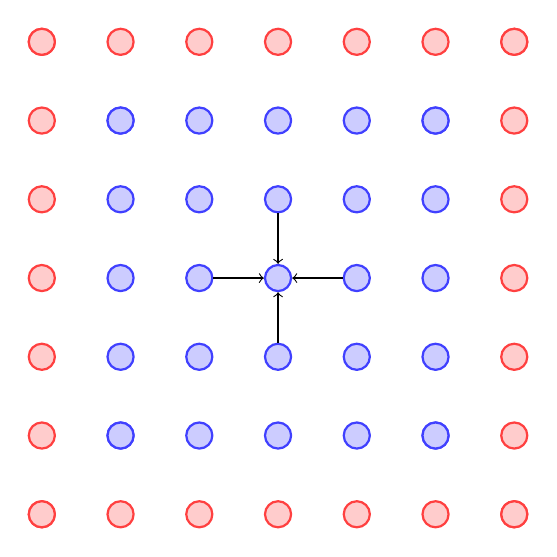
\begin{tikzpicture}
\tikzstyle{place}=[circle,thick,draw=blue!75,fill=blue!20,minimum size=2mm]

\node[place] (p1) at (0,0) {};
\node[place] (p2) at (0,1) {};
\node[place] (p3) at (1,0) {};
\node[place] (p4) at (-1,0) {};
\node[place] (p5) at (0,-1) {};

\node[place] () at (-1,-1) {};
\node[place] () at (-1,1) {};
\node[place] () at (1,-1) {};
\node[place] () at (1,1) {};

\foreach \x in {-2,...,2}
{
  \node[place] () at (\x,2) {};
  \node[place] () at (\x,-2) {};
  \node[place] () at (2,\x) {};
  \node[place] () at (-2,\x) {};
}

\draw[->] (p2) to (p1);
\draw[->] (p3) to (p1);
\draw[->] (p4) to (p1);
\draw[->] (p5) to (p1);

\tikzstyle{place}=[circle,thick,draw=red!75,fill=red!20,minimum size=2mm]

\foreach \x in {-3,...,3}
{
  \node[place] () at (\x,3) {};
  \node[place] () at (\x,-3) {};
  \node[place] () at (3,\x) {};
  \node[place] () at (-3,\x) {};
}



\end{tikzpicture}
}
\end{figure}

L'utilisation courante des stencils dans les algorithmes scientifiques a conduit à des bibliothèques de type DSEL comme \textsf{Pochoir} \cite{Art18} ou  \textsf{Blitz++} \cite{Art5}, et des langages de type DSL tels que \cite{Art19}, qui -- hormis \textsf{Blitz++} -- nécessitent leur propre compilateur afin d'effectuer des optimisations. Toutefois les stencils sont aussi utilisées dans des applications physiques non scientifiques, par exemple dans le calcul des graphismes de jeux vidéos \cite{Art15}. Dans les deux cas la performance est primordiale et il est donc nécessaire d'exploiter les possibilités de parallélisme des machines utilisées pour ces calculs.  

Si l'on suppose que la mise à jour de la grille par application du stencil n'est pas calculée en place -- c'est-à-dire que l'on dispose d'un tableau d'entrée dans lequel les éléments sont seulement lus, et d'un tableau de sortie où les résultats du calcul du stencil sur chaque élément sont stockés -- le stencil peut être appliqué à chaque élément bleu en même temps. Le parallélisme se trouve donc de manière très aisée dans ce type de problème. Avec une  machine possédant autant de cœurs que d'éléments dans la grille, la mise à jour de la grille se fait donc en une seule étape et tous les processeurs exécutent les mêmes instructions, simplement sur des éléments différents ; le calcul est donc bien adapté à une carte graphique qui regroupe justement ces caractéristiques : nombre élevé de cœurs et un même code s'exécutant sur tous ceux-ci. Puisque le calcul n'est pas en place, pour l'appliquer plusieurs fois d'affiliés il suffit d'intervertir les grilles d'entrées et de sortir entre chaque mise à jour, ou bien de recopier la sortie vers l'entrée, ce qui est toutefois plus lent. Par ailleurs le parallélisme peut s'obtenir grâce à l'architecture superscalaire des processeurs : par exemple pour la mise à jour des éléments de toute une ligne en même temps sur l'exemple précédent, il suffit de faire quatre additions superscalaires : la ligne est sommée avec celle du dessus, celle du dessous, elle-même décalée d'un élément vers la gauche, elle-même décalée d'un élément vers la droite. Il y a donc possibilité de parallélisme à plusieurs niveaux du matériel : intraprocesseur et interprocesseur. 

Le parallélisme s'obtient donc immédiatement pour les stencils, mais cela ne signifie pas pour autant qu'il est efficace. En effet les problèmes qui les utilisent nécessitent généralement beaucoup de mémoire (qui est de plus doublée en considérant que les calculs ne sont pas en place), ce qui rend l'efficacité moindre. La mémoire des ordinateurs est hiérarchique et les lectures/écritures rapides des éléments d'une grille ne peuvent se faire que sur de petites parties proches des processeurs. Il s'agit de la mémoire \emph{cache} -- ou plus simplement, du cache -- qui est elle-même hiérarchique. Les plus grandes difficultés dans la parallélisation des stencils sont ainsi liées à la bonne utilisation de la mémoire, afin d'éviter les chargements/déchargements inutiles de données. En effet si nous supposons que chaque cœur est associé à un élément de la grille et en considérant de nouveau le cas de la figure \ref{fig:stencil_base}, chaque élément nécessite les valeurs des quatre éléments autour de lui pour effectuer le calcul. Si chaque cœur chargeait séparément ces valeurs, il faudrait donc l'équivalent de cinq grilles en mémoire (quatre -- identiques -- pour les valeurs de départ et une pour le résultat), alors qu'en réalité seule deux sont nécessaires. La difficulté de la parallélisation des stencils réside donc dans la façon d'utiliser la mémoire, notamment en faisant en sorte que les cœurs soient disposés comme les éléments de la grille et partagent avec leurs voisins les éléments qu'ils utilisent, afin d'une part de maximiser la réutilisation des données, et d'autre part de minimiser les temps de transfert.

L'élément premier de la hiérarchie de la mémoire est le disque dur, qui est suivi par la mémoire RAM plus rapide mais plus petite. Nous supposons ici que le problème peut toujours être contenu en mémoire RAM. C'est alors la mémoire des processeurs qui pose problème : le cache. Lui même est décomposé en plusieurs niveaux suivant (de la RAM vers les cœurs) qui sont de plus en plus petits et rapides, mais de moins en moins partagés. La figure \ref{fig:memoire_base} donne un exemple de cette hiérarchie pour deux processeurs et une carte graphique. Les caches des processeurs possèdent trois niveaux dont les deux derniers sont exclusifs tandis que le premier est partagé de manière directe entre les cœurs d'un même processeurs, il est même partagé entre tous les cœurs mais avec un accès \emph{non-uniforme}. Chaque processeur central est alors appelé un nœud NUMA et l'accès au cache de l'autre est plus coûteux que l'accès au sien. Quant au processeur graphique il possède une mémoire globale assez grande, et des petites mémoires partagées par des groupes -- ou \emph{warps} -- de $16$ ou $32$ cœurs. Cette mémoire n'est pas un cache pour le processeur graphique, car celui-ci n'opère pas de cohérence des données entre les cœurs : c'est au programmeur de savoir quel cœur possède la donnée la plus à jour. Il en résulte une plus grande complexité dans la gestion de la mémoire graphique, et notamment l'obligation d'avoir de temps en temps des synchronisations entre les cœurs d'un même warp. 

\begin{figure}[!h]
  \caption{Exemple de structure hiérarchique de la mémoire (en vert) d'un ordinateur possédant deux processeurs et une carte graphique (les cœurs de calcul sont en rouge).}
  \label{fig:memoire_base}
  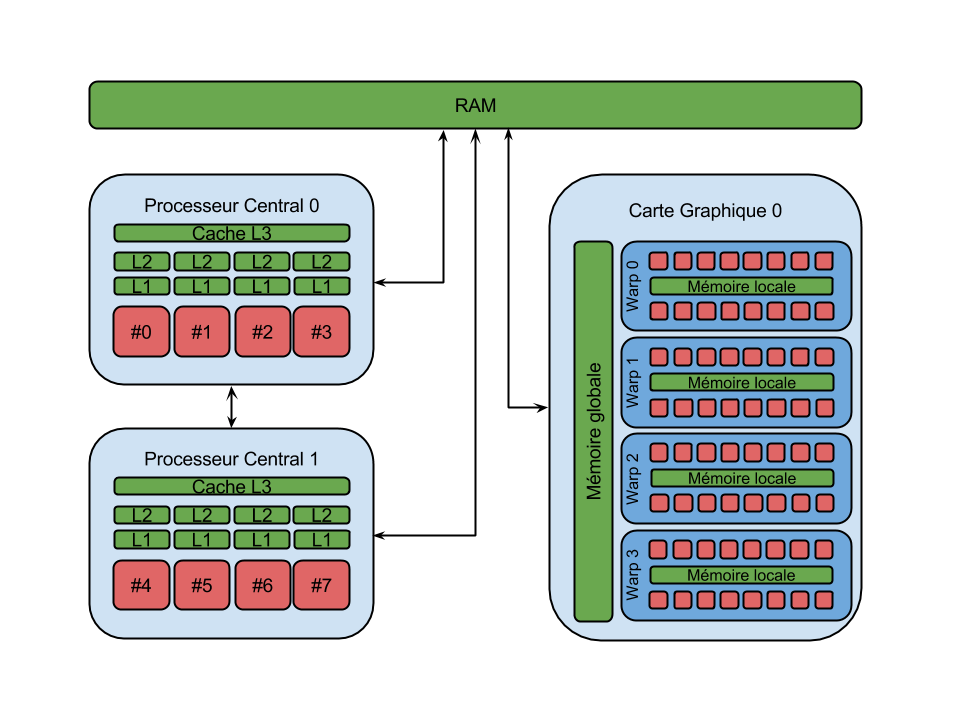
\includegraphics[width=\textwidth]{Memory.png}
\end{figure}


\section{Conception d'un DSEL pour les stencils}

Principalement deux DSEL existent déjà pour les stencils : \textsf{Pochoir} et \textsf{Blitz++} cependant les deux souffrent de plusieurs désavantages. Les deux nécessitent l'apprentissage de plusieurs mots-clés qui fonctionnent généralement comme des balises HTML : ils ouvrent des sections spécifiques puis les ferment. Cela facilite certainement l'analyse du code par le compilateur dans le cas de \textsf{Pochoir}, mais dans les deux cas cela est contraire au paradigmes assez répondu de l'utilisation de fonctions à arguments (ou bien méthodes) pour initialiser ou faire des calculs sur des éléments (objets, structures, etc\ldots) -- que ce soit dans la programmation orientée objet, impérative ou fonctionnelle. Par ailleurs \textsf{Blitz++} souffre de l'utilisation de \emph{macros}, des parties de codes qui sont rajoutées dans le code par le compilateur avant la compilation, mais sont parfois présentées comme des fonctions au développeur ; en cas d'erreur lors de la compilation il peut donc il y avoir confusion sur son origine. Enfin les deux DSEL se focalisent sur une exécution sur CPU uniquement, alors que les GPU sont très adaptés à ce genre d'opérations.

Todd L. Veldhuizen, le concepteur de \textsf{Blitz++}, a introduit la notion d'\emph{active libraries} (\emph{bibliothèques actives}) \cite{Art20} afin de décrire ce qu'un DSEL notamment (ainsi que le compilateur associé) doit proposer a minima. Ces bibliothèques doivent tirer partie de toutes les possibilités dont elles disposent : à la fois la sémantique de l'expression qui est codée par le biais du DSEL, et à la fois les performances offertes par des bibliothèques spécialisées dans certains types d'opérations. Elles sont actives car elles ne fournissent pas seulement des méthodes optimisées, elles les choisissent en fonction de l'expression. Par ailleurs Todd Veldhuizen propose dans l'article \cite{Art22} trois aspects à développer dans le DSEL afin d'obtenir des performances : \emph{Pretty, Safe, Fast} (pour joli, sûr, et rapide). Ces trois aspects sont au centre des préoccupations avec lesquelles le DSEL a été développé au cours du stage. Tandis que nous regroupons le caractère joli et sûr dans les objectifs sémantiques, la rapidité est quant à elle liée à la performance.

\subsection{Objectifs sémantiques}

Le premier objectif sémantique est tout simplement de pouvoir décrire toutes les formes de stencils. Le stencil lui-même est déterminé par les indices des éléments qui rentrent en jeu dans le calcul. Dans l'exemple précédent de stencil à quatre points dans une grille en deux dimensions, si nous considérons comme origine du repère un élément quelconque à mettre à jour alors les éléments nécessaires à sa mise à jour sont d'indices $(-1,0)$, $(1,0)$, $(0,-1)$ et $(0,1)$. La simple connaissance de ces indices relatifs permet de retrouver le motif du stencil, il est donc primordial de pouvoir déclarer simplement les indices entrant en jeu dans le stencil. Dans la suite du document nous appelons ces indices relatifs les \emph{indices de décalage}.

Par ailleurs un stencil peut nécessiter des coefficients. Par exemple dans le cas de l'algorithme classique Jacobi, ces coefficients sont constants et ne sont liés qu'aux positions relatives des éléments accédés par le stencil. Si la grille des éléments est stockée dans un tableau $A$ à deux dimensions, l'équation associée à la mise à jour d'un élément d'indice global $(i,j)$ par le stencil pourrait donc s'écrire de façon mathématique comme l'équation \ref{eq:st0_fxd} où les $c_x$ sont les coefficients fixes.
\begin{equation}
\label{eq:st0_fxd}
A[i,j] = c_1 \times A[i-1,j+0] + c_2 \times A[i+1,j+0] + c_3 \times A[i+0,j-1] + c_4 \times A[i+0,j+1]
\end{equation}
Les coefficients étant dans ce cas liés aux indices de décalage, un DSEL doit donc permettre la possibilité de déclarer les deux en même temps.

Toutefois cet exemple ne regroupe pas tous les cas possibles, il est par exemple possible d'imaginer abstraire l'opération de réduction qu'est ici la somme -- ce qui n'est pas très utile --, de même que l'opération liant les coefficients aux éléments de la grille -- ce qui est beaucoup plus utile par exemple si les éléments ne sont pas de simples scalaires, mais des matrices ou des nombres complexes. Nous notons respectivement $\oplus$ et $\otimes$ ces deux opérations, l'équation \ref{eq:st0_fxd} se réécrit alors en l'équation \ref{eq:st1_fxd}.
\begin{equation}
\label{eq:st1_fxd}
A[i,j] = c_1 \otimes A[i-1,j+0] \oplus c_2 \otimes A[i+1,j+0] \oplus c_3 \otimes A[i+0,j-1] \oplus c_4 \otimes A[i+0,j+1]
\end{equation}
La nature des opérateurs doit donc apparaître dans la définition du stencil.

Une autre variante sur les coefficients consiste à les considérer variables en fonction non seulement de l'élément calculé, mais aussi en fonction du décalage pour chaque élément entrant en compte. Une telle possibilité est parfois utile, notamment dans les calculs de chromodynamique quantique. Nous notons $f$ la fonction qui renvoie le coefficient en fonction des différents indices (celui de l'élément traité, et celui des éléments utilisés). En deux dimensions $f$ prend donc quatre arguments et l'équation \ref{eq:st1_fxd} devient l'équation \ref{eq:st1_var}.
\begin{equation}
\label{eq:st1_var}
\begin{aligned}
A[i,j] = & f(i, j, -1,  0) \otimes A[i-1,j+0] \oplus \\
         & f(i, j,  1,  0) \otimes A[i+1,j+0] \oplus \\
         & f(i, j,  0, -1) \otimes A[i+0,j-1] \oplus \\ 
         & f(i, j,  0,  1) \otimes A[i+0,j+1]
\end{aligned}
\end{equation}

Cette dernière équation est un peu plus complexe à abstraire car les coefficients ne sont plus seulement liés aux indices relatifs de décalage. En effet le stencil est alors défini par une fonction supplémentaire, et la déclaration d'une telle fonction peut-être laborieuse. Pour rendre cette fonction plus simple à déclarer, $f$ devient alors une fonction d'accès uniquement qui au lieu de déterminer la valeur du coefficient grâce au paramètre, permet d'accéder à l'endroit où se situe le coefficient pré-calculé dans un tableau. La déclaration de $f$ est alors plus aisée, mais le stencil nécessite également la connaissance du tableau de coefficients (que l'utilisateur doit lui-même pré-remplir). $f$ prend alors un cinquième argument (le tableau) noté $C$.

Ce choix d'avoir un tableau supplémentaire, permet d'ailleurs d'abstraire la structure des données, et il serait souhaitable de l'utiliser non seulement pour les coefficients variables, mais aussi pour les éléments de la grille de calcul. Cette fonction $g$ prend alors en argument l'indice -- non-relatif, global -- de l'élément courant ainsi que le tableau de la grille. De cette façon la grille peut être stockée sous une forme entièrement paramétrable : \emph{row major}\footnote{Dans le cas d'une grille à deux dimensions, la disposition \emph{row major} consiste à placer les lignes les unes à la suite des autres dans un tableau à une dimension.}, \emph{column major}\footnote{Idem note précédente, par colonne.} ou autre. On peut alors réécrire la dernière équation, en considérant maintenant le fait que le calcul ne se fait pas en place et que le résultat est stocké dans un tableau $B$, et l'on obtient l'équation \ref{eq:st2_var}.
\begin{equation}
\label{eq:st2_var}
\begin{aligned}
g(i,j,B) = & f(i, j, -1, \quad 0, C) \otimes g(i-1, j+0, A) \, \oplus \\
           & f(i, j, \quad 1, \quad 0, C) \otimes g(i+1,j+0, A) \, \oplus \\
           & f(i, j, \quad 0, -1, C) \otimes g(i+0,j-1, A) \, \oplus \\ 
           & f(i, j, \quad 0, \quad 1, C) \otimes g(i+0,j+1, A)
\end{aligned}
\end{equation}

En résumé l'application d'un stencil sur une grille nécessite l'enregistrement dans le DSEL des éléments suivants : 
\begin{itemize}
\item les indices de décalage (avec éventuellement les coefficients constants) ;
\item la fonction d'accès aux coefficients variables et le tableau associé (s'il n'y a pas de coefficients constants) ;
\item les opérateurs de réduction $\oplus$ et d'application du coefficient à l'élément $\otimes$ ;
\item les tableaux d'entrées et sorties ;
\item la fonction d'accès pour ces deux tableaux.
\end{itemize}

Éventuellement, le DSEL peut prévoir plusieurs types d'agrégations :
\begin{itemize}
\item la combinaison de plusieurs motifs de stencils en un seul ;
\item la possibilité d'appliquer le même motif sur plusieurs tableaux à la fois ;
\item le \emph{stream} (ou \emph{flux}) de plusieurs stencils à la suite sur un unique tableau de départ, les tableaux intermédiaires étant alors omis.
\end{itemize}

Les caractères joli et sûr du DSEL sont nécessairement dépendant du langage choisi. En ce qui concerne l'élégance, il s'agit d'utiliser le moins de symboles et fonctions possibles, et de cacher tous les paramètres inutiles. Pour la sûreté le but est de détecter certains types d'erreurs comme l'utilisation du même tableau en entrée et en sortie (en supposant que le calcul en place n'a pas lieu d'être) et l'usage d'indices de décalage en dehors de la grille.

\subsection{Objectifs de performances}

Les performances peuvent s'obtenir grâce à l'adaptation du code tant par rapport au matériel que par rapport aux algorithmes de calculs utilisés. Deux voies principales doivent être explorées : la réutilisation maximale des données dans le cache (qui induit le principe de \emph{tuilage}), le calcul du plus grand nombre de paramètres possibles lors de la compilation (les variables en jeu étant alors \emph{statiques}).

\subsubsection*{Tuilage de stencil} 

Avant de déterminer quels paramètres peuvent être calculés à la compilation, il est nécessaire de voir plus en détail comment la parallélisation va être effectuée au sein du stencil. Puisque les tableaux utilisés dans les calculs sont généralement trop grand pour la mémoire respectivement cache ou locale proche des processeurs respectivement centraux ou graphiques, la grille de l'exemple précédent est divisée en blocs que nous appelons \emph{macro-tuiles}. La taille de chaque macro-tuile est choisie de façon que la mémoire utilisée par les calculs tienne soit dans les caches L3 soit dans la mémoire locale (cf figure \ref{fig:memoire_base}). La façon de paralléliser la macro-tuile est la suivante : chaque processeur central (ou warp dans le cas des cartes graphiques) est lié à une macro-tuile et chaque cœur va appliquer le stencil sur un ou plusieurs éléments différents\footnote{La notion de \emph{tuile} sera utilisée dans la section \ref{sec:desc_mat_tests} et fait référence à la parallélisation au sein d'un cœur, et non au sein d'un processeur.}. Si l'on reprend l'exemple de la figure \ref{fig:memoire_base} avec le stencil à $4$ points, la parallélisation par tuilage sur la carte graphique sur une grille de $10$ par $10$ éléments va pouvoir se faire en la découpant en quatre blocs carrés chacun associé à un warp. Chaque \emph{warp} possédant chacun $16$ cœurs va appliquer le stencil sur une macro-tuile de dimensions $4 \times 4$. La figure \ref{fig:stencil_mtile} représente cette situation en précisant par des bordures en pointillées les éléments fantômes que le \emph{warp} $0$ coloré en jaune devra contenir. Bien que les seuls fantômes à la base soient les éléments rouges en bordure de la grille, chaque \emph{warp} a besoin de charger les éléments autour de lui compte-tenu de la forme du stencil.

\begin{figure}[!h]
\floatbox[{\capbeside\thisfloatsetup{capbesideposition={right,center},capbesidewidth=4cm}}]{figure}[\FBwidth]
{\caption{Exemple de tuilage d'une grille en deux dimensions sur une carte graphique possédant $4$ \emph{warps} Les éléments calculés sont en bleus, les fantômes en rouges et dans les cadres pointillés.}\label{fig:stencil_mtile}}
{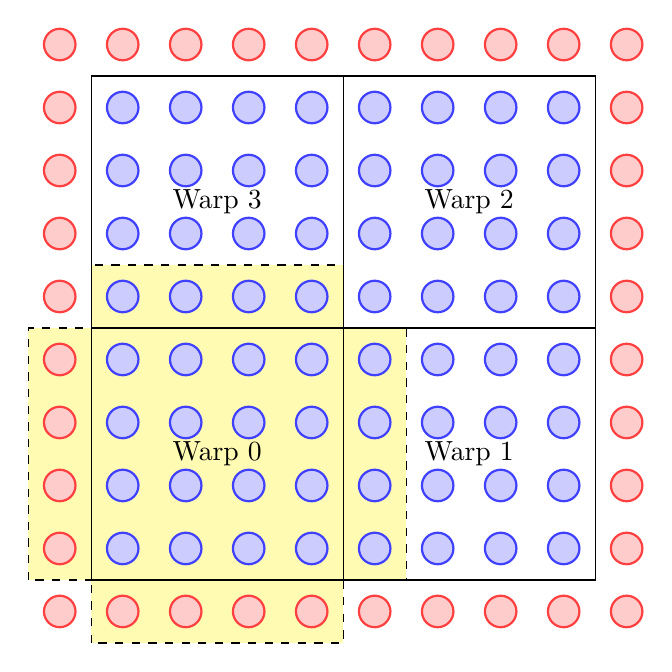
\begin{tikzpicture}[scale=0.8]
\tikzstyle{place}=[circle,thick,draw=blue!75,fill=blue!20,minimum size=4mm]

\draw[dashed,fill=yellow!30] (0.5,-0.5) rectangle (4.5,0.5);
\draw[dashed,fill=yellow!30] (-0.5,0.5) rectangle (0.5,4.5);
\draw[dashed,fill=yellow!30] (0.5,4.5) rectangle (4.5,5.5);
\draw[dashed,fill=yellow!30] (4.5,0.5) rectangle (5.5,4.5);

\draw[fill=yellow!30] (0.5,0.5) rectangle (4.5,4.5);
\draw (4.5,4.5) rectangle (8.5,8.5);
\draw (0.5,4.5) rectangle (4.5,8.5);
\draw (4.5,0.5) rectangle (8.5,4.5);


\foreach \x in {1,...,8}
{
  \foreach \y in {1,...,8}
  {
    \node[place] () at (\x,\y) {};
  }
}

\node () at (2.5,2.5) {Warp 0};
\node () at (6.5,2.5) {Warp 1};
\node () at (6.5,6.5) {Warp 2};
\node () at (2.5,6.5) {Warp 3};


\tikzstyle{place}=[circle,thick,draw=red!75,fill=red!20,minimum size=4mm]

\foreach \x in {0,...,9}
{
  \node[place] () at (\x,0) {};
  \node[place] () at (\x,9) {};
}
\foreach \y in {1,...,8}
{
  \node[place] () at (0,\y) {};
  \node[place] () at (9,\y) {};
}



\end{tikzpicture}
}
\end{figure}

L'intérêt du tuilage est de pouvoir faire rentrer tous les éléments nécessaires à la mise-à-jour d'une macro-tuile dans le cache L3 (ou la mémoire locale) du processeur (ou du warp) qui la traite. De plus nous ne perdons pas en parallélisation (dans l'exemple précédent tous les éléments sont calculés en même temps puisqu'il y a autant d'éléments que de cœurs). La gestion de la mémoire n'est cependant pas parfaite, puisque chaque macro-tuile nécessite sa zone fantôme dont les éléments ne seront utilisés qu'une seule fois. D'autres formes de découpage que les blocs carrés existent, afin de minimiser cette zone fantôme suivant la forme du stencil, ce point sera évoquée à la section \ref{sec:evol_biblio}.

Le cas de la figure \ref{fig:stencil_mtile} est simple car il y a autant de cœurs que d'éléments à calculer, il reste donc à gérer le cas général où la grille de base est beaucoup plus grande que le nombre de cœurs, et dont les dimensions n'en sont pas forcément des multiples entiers d'ailleurs. En pratique les macro-tuiles vont alors être calculées les unes après les autres. Et si les dimensions de la grille ne sont multiples du nombres de processeurs, les macro-tuiles dont certains éléments dépassent de la grille ne seront pas calculés, par l'intervention de condition sur la taille globale. 

De même cet exemple est uniquement en deux dimensions, mais certains calculs nécessitent des stencils sur des grilles à quatre dimensions, notamment en chromodynamique quantique. Certains articles \cite{Art1,Art11} développent des techniques spécifiques pour y remédier, tout en gardant une certaine réutilisation des données. Ces techniques sont très spécialisées et ne seront pas évoquées ici, toutefois il convient de savoir qu'elles existent et que le DSEL devrait être capable à terme de les intégrer.

\subsubsection*{Variables statiques}

Les variables statiques vont permettre d'éviter au programme certains calculs lors de l'exécution (qui sont alors reportés à l'exécution), et donc d'être légèrement plus rapide. Les principales variables entrant en jeu pour la parallélisation sont :
\begin{itemize}
\item le nombre de dimensions de la grille ;
\item le nombre d'éléments dans chaque dimension de la grille ;
\item le nombre d'éléments du stencil ;
\item les indices de décalage du stencil ;
\item la taille des zones fantômes de la grille ;
\item la quantité de mémoire disponible en mémoire cache de niveau 3 ou en mémoire locale ;
\item le nombre de processeurs et cœurs disponibles à l'intérieur ;
\item la forme et la taille des macro-tuiles ;
\item la taille des zones fantômes des macro-tuiles.
\end{itemize}

Toutes ces variables peuvent (et doivent) être statique hormis le nombre d'éléments de la grille, qui par choix est déterminé à l'exécution. En effet nous supposons que le programme doit être compilé pour chaque problème différent (donc avec des stencils différents) mais pas pour chaque instance du même problème, où seul le nombre d'éléments (donc la précision de la résolution) change. C'est cette approche qui est aussi utilisée dans \textsf{QIRAL}. Le problème est alors de savoir comment calculer ces variables statiquement -- certaines peuvent se déduire les unes des autres --, et cela dépend du langage choisi pour le DSEL, notamment si le langage autorise la méta-programmation, une façon de modifier le comportement de certaines fonctions à la compilation. Le calcul de la taille des macro-tuiles et de leur zone fantôme est détaillé dans la section \ref{sec:param_tuile} du chapitre suivant.

Plus généralement, d'autres variables aidant dans l'ordonnancement des calculs (notamment si plusieurs types de processeurs sont disponibles) pourraient (mais difficilement) être calculées lors de la compilation, mais cela n'a pas été étudié dans le cadre du stage, d'autant que la tendance actuelle est justement à l'opposée : c'est le rôle des supports d'exécutions que de faire ces calculs lors de l'exécution. Outre l'ordonnancement des calculs, il s'agit aussi d'ordonnancer les recopies mémoires, notamment vers la mémoire globale des processeurs graphiques.

